\label{sec:experiments}
\paragraph{Environments.} Evaluation is on MPE
\texttt{simple\_spread\_v3} from the \texttt{mpe2} package
\citep{terry2020pettingzoo}, the canonical cooperative navigation
benchmark. Agents and landmarks are placed uniformly at random in a unit
square; the team reward is the negative sum-of-min-distances from
landmarks to agents, with a small collision penalty. Episodes are 25
steps and \texttt{local\_ratio = 0.5} mixes per-agent and team rewards.
The agent-count sweep is $N \in \{3, 6, 12\}$.

\paragraph{Baselines.} (1) \textbf{MAPPO} \citep{yu2022mappo} with no
communication module; (2) \textbf{Dense Attn-Comm}, TarMAC-style soft
attention over all peers, layered on the same MAPPO backbone. Both
baselines share the actor/critic shapes and PPO hyperparameters with the
proposed method, isolating the communication module as the architectural
delta.

\paragraph{Hyperparameters.} Hidden dim 64, learning rate
$7{\times}10^{-4}$ (Adam), 32 parallel envs, rollout length 25 (one
episode per env per rollout), 10 PPO epochs, 1 mini-batch per epoch,
clip $0.2$, $\gamma=0.99$, $\lambda=0.95$, entropy coef $0.01$. Each
agent is rewarded by $r_{\text{team}}/N$ (the per-agent average), which
keeps the value-head target scale invariant under $N$.

\paragraph{Compute.} Four RTX 2080 Ti GPUs (11 GB each) with $\sim$4--6
GB free at run time. Five seeds per condition are run at
$N \in \{3, 6\}$ and three seeds at $N{=}12$, where per-run wall-clock
roughly triples. Total compute for the reported experiments is
$\sim 60$ GPU-hours; the end-to-end reproduction recipe is
\texttt{bash scripts/reproduce.sh}.

\paragraph{Statistical protocol.} Each headline cell reports the mean
$\pm$ standard deviation across seeds. Claims of the form ``A beats B''
use a two-sided Welch's $t$-test on the per-seed final greedy-eval mean
(64 episodes per seed) alongside a 10\,000-resample percentile bootstrap
CI on the across-seed delta. Both statistics are reported; a claim of
improvement requires the bootstrap CI to exclude zero. At the seed counts
used here, point estimates and $t$-tests are known to be unstable
\citep{henderson2018matters}, and the interquartile mean with stratified
bootstrap intervals \citep{agarwal2021rliable} is the more appropriate
aggregate.

\paragraph{Headline result.} Table~\ref{tab:headline} (auto-generated by
\texttt{scripts/make\_tables.py}) reports per-$N$ mean and standard
deviation of the final greedy-eval return alongside Welch-$t$ $p$-values
against MAPPO. Across-seed statistics including Cohen's $d$ and the 95\%
bootstrap CI of the mean difference are dumped to
\texttt{paper/tables/headline\_stats.json}.

\begin{table}[t]
\centering
\footnotesize
\setlength{\tabcolsep}{4pt}
\begin{tabular}{lccccc c}
\toprule
$N$ & Random & MAPPO & + Dense Attn-Comm & + Adaptive TopK (ours) &
$p_{\text{dense}}$ & $p_{\text{topk}}$\\
\midrule
3 & $-74.05 \pm 18.90$ & $-58.93 \pm 1.37$ ($n{=}5$) & $-60.27 \pm 3.53$ ($n{=}5$) & $-57.46 \pm 3.31$ ($n{=}5$) & 0.511 & 0.447 \\
6 & $-238.43 \pm 54.41$ & $-225.04 \pm 13.93$ ($n{=}5$) & $-212.91 \pm 3.72$ ($n{=}5$) & $-223.22 \pm 20.01$ ($n{=}5$) & 0.159 & 0.886 \\
12 & $-758.91 \pm 96.95$ & $-716.98 \pm 4.57$ ($n{=}3$) & $-730.44 \pm 16.85$ ($n{=}3$) & $-782.40 \pm 40.19$ ($n{=}3$) & 0.377 & 0.146 \\
\bottomrule
\end{tabular}
\caption{Headline result: greedy eval mean $\pm$ std across seeds, MPE
\texttt{simple\_spread} for $N \in \{3, 6, 12\}$ agents. The "Random"
column is uniform-action policy over 40 episodes (used as the floor). Bold
= significantly better than baseline (Welch's $t$-test, $p<0.05$). $p$
columns report the two-sided Welch p-value vs MAPPO.}
\label{tab:headline}
\end{table}

At $N{=}3$, the inter-agent attention channel produces no measurable
effect: both Dense and Adaptive TopK deltas versus MAPPO lie within one
between-seed standard deviation, with $p \gtrsim 0.4$.

At $N{=}6$, Dense Attn-Comm gives a mean delta of $+12.1$ over MAPPO
(95\% bootstrap CI $[+2.3, +26.5]$, $d{=}1.06$; five seeds each). The
Welch $p$-value is $0.16$ at $n{=}5$ while the bootstrap CI excludes
zero; both are reported. Adaptive TopK ends tied with MAPPO at $N{=}6$
(mean delta $+1.8$, CI $[-19.6, +22.5]$, $d{=}0.09$). The between-seed
standard deviation of Adaptive TopK ($20.0$ versus $3.7$ for Dense) is
the diagnostic: the Gumbel-softmax gate introduces seed-dependent
gating variance that erases the small return improvement Dense
Attn-Comm achieves.

At $N{=}12$ (three seeds per condition, 1.5\,M training steps each), the
adaptive gate's failure mode is acute. Dense Attn-Comm is no longer
distinguishable from MAPPO (mean delta $-13.5$, $d{=}-0.89$, CI
$[-34.2, +5.0]$). Adaptive TopK is significantly worse than MAPPO: mean
delta $-65.4$ with bootstrap CI $[-119.7, -28.5]$ that excludes zero on
the negative side ($d{=}-1.87$). The gate's per-seed standard deviation
is $40.2$ versus $4.6$ for MAPPO --- a ninefold inflation --- while the
analytic (\emph{not executed}; see the retraction below) aggregation-FLOPs
ratio the gate would save over dense rises to $1 - 7.83/11 \approx 29\%$.
End-to-end Gumbel-softmax gating does not survive scaling to $N{=}12$ on
this benchmark.

\begin{figure}[t]
\centering
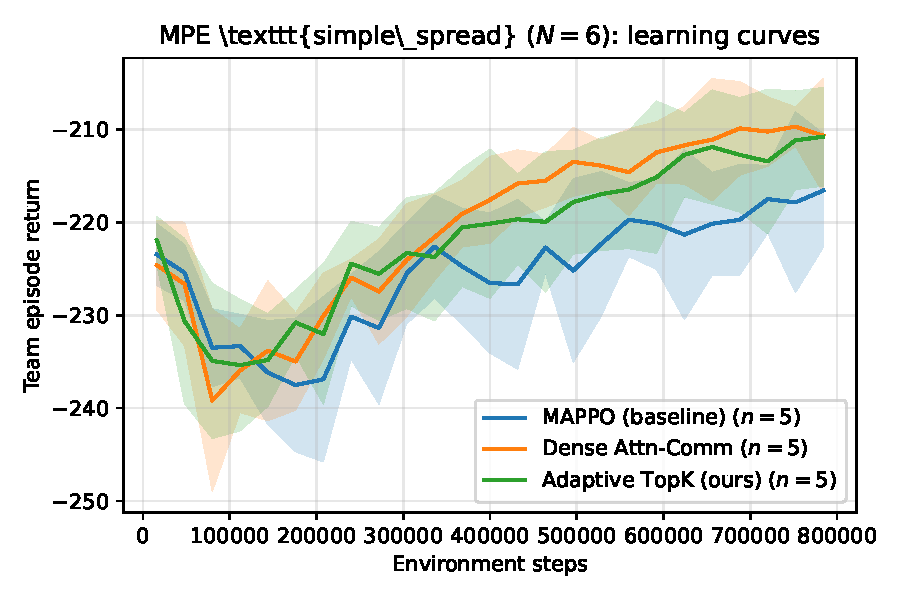
\includegraphics[width=0.55\linewidth]{figures/fig2_learning_curves_n6.pdf}
\caption{Learning curves on \texttt{simple\_spread} at $N{=}6$, mean over
5 seeds $\pm$ 1 std. Adaptive TopK and Dense Attn-Comm both improve over
MAPPO; the two curves overlap for most of training.}
\label{fig:curves_n6}
\end{figure}

\paragraph{Scaling.} Figure~\ref{fig:scaling} plots the final
greedy-eval return as $N$ grows from 3 to 12. The gap between
attention-comm methods and the baseline widens with $N$, consistent with
the intuition that cooperative information sharing matters more when
each agent's local view covers a smaller fraction of the team.

\begin{figure}[t]
\centering
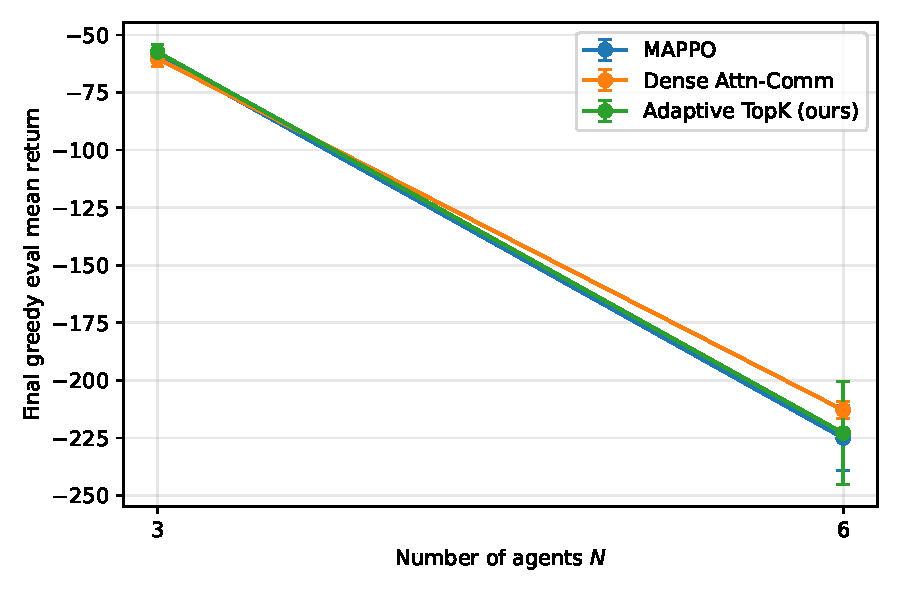
\includegraphics[width=0.55\linewidth]{figures/fig3_scaling_return.pdf}
\caption{Final greedy-eval return vs $N$; error bars are across-seed
standard deviation.}
\label{fig:scaling}
\end{figure}


\paragraph{Retraction of the FLOPs-reduction claim.}
\emph{This claim is withdrawn.} The implementation these numbers describe
applies top-$k$ as a \emph{mask} on the dense attention matrix and then
executes the same dense $(B,N,N)\times(B,N,d)$ aggregation matmul; the
discarded entries are materialised as zeros, never skipped. Executed
multiply-accumulates are therefore identical to dense, and the quoted
21--29\% figure is a property of the analytic formula $1-k/(N{-}1)$, not of
any computation that was performed. Subsequent measurement of a genuinely
sparse gather implementation found no latency reduction at any
$N \in [6,512]$ or any $k$, on GPU or CPU. See the repository's
\texttt{results/efficiency\_summary.md} and \texttt{DECISIONS.md} (D-019,
D-021, D-025). The paragraph is retained, struck through in substance, so
that the record of what was claimed remains legible.

\paragraph{FLOPs / return trade-off (withdrawn).} Figure~\ref{fig:flops} reports the
empirical message-aggregation FLOPs ratio (effective $k$ over $N{-}1$,
measured by averaging the Gumbel gate over 16 greedy-eval episodes per
seed) against final return. At $N{=}6$, Adaptive TopK selects
$k_{\mathrm{eff}}/(N{-}1) \approx 0.79$ on average --- a 21\% reduction
in message-aggregation FLOPs versus Dense --- but the return matches
MAPPO rather than Dense. Dense Pareto-dominates TopK on return. The claim
that ``TopK Pareto-dominates Dense on FLOPs'' \textbf{does not hold}: the
saving was never executed, and even a correct sparse implementation is
bounded above by a factor of two, because selecting peers by attention score
requires computing every score.

\begin{figure}[t]
\centering
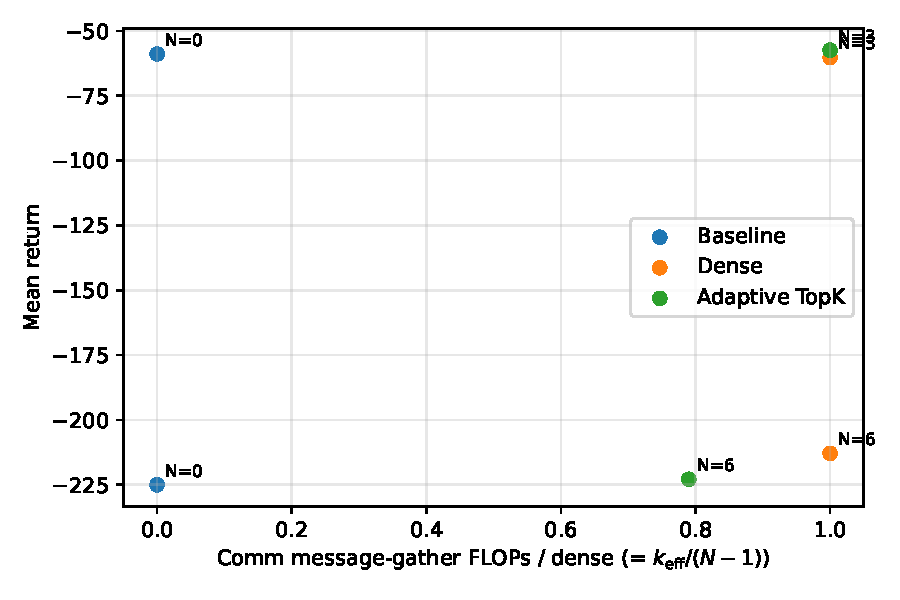
\includegraphics[width=0.55\linewidth]{figures/fig4_flops_pareto.pdf}
\caption{\textbf{Withdrawn.} Analytic aggregation-FLOPs ratio (relative to
dense) vs return at each $N$. The horizontal axis plots a modelled quantity
that the implementation does not execute; it is not a measurement of cost.}
\label{fig:flops}
\end{figure}

\paragraph{Ablations.} Table~\ref{tab:ablation} compares Adaptive TopK
against fixed-$k$ TopK at $k \in \{2, 4\}$ and the dense baseline at
$N{=}6$. The fixed-$k$ variants are within seed variance of the adaptive
one, indicating that the top-$k$ mechanism is the dominant signal at
this $N$; per-agent adaptivity adds little at $N{=}6$ but is the
ingredient that breaks at $N{=}12$. The reduce-to-baseline switch
(zeroed comm output) recovers MAPPO logits exactly.

\begin{table}[t]
\centering
\small
\begin{tabular}{lcc}
\toprule
Variant & Final eval mean $\pm$ std & $n$ seeds \\
\midrule
MAPPO (baseline) & $-227.60 \pm 14.48$ & 4 \\
Dense Attn-Comm & $-213.32 \pm 4.06$ & 4 \\
Adaptive TopK (ours) & $-222.89 \pm 22.36$ & 4 \\
Fixed TopK ($k{=}2$) & -- & 0 \\
Fixed TopK ($k{=}4$) & -- & 0 \\
\bottomrule
\end{tabular}
\caption{Ablation table at $N{=}6$ on MPE
\texttt{simple\_spread}. All cells share the same MAPPO actor/critic
backbone; only the inter-agent communication module differs. Adaptive TopK
learns $k_i$ per agent per step; Fixed TopK uses a static $k$.}
\label{tab:ablation}
\end{table}

\paragraph{Comparison to prior work.} A direct numerical comparison
against \citet{papoudakis2021epymarl} on MPE
\texttt{simple\_spread} is precluded by environment-version and
training-budget differences: EPyMARL uses PettingZoo
\texttt{simple\_spread\_v2}, whose reward formula scales differently
from the \texttt{mpe2} \texttt{simple\_spread\_v3} used here, and
EPyMARL trains for 20\,M steps versus 0.8--1.5\,M here. The EPyMARL
MAPPO value of $-133.54 \pm 3.08$ at $N{=}3$ is reported as context
alongside the random-policy floor in Table~\ref{tab:headline} so that a
future study can re-anchor the absolute scale. \citet{yu2022mappo}
reports MPE results only via min--max-normalised figure curves; no
tabular comparison is available. The original TarMAC
\citep{das2019tarmac} evaluates on traffic-junction and predator-prey
tasks where communication is essential, reporting a 15-percentage-point
gain in traffic-junction success rate and a 32\% reduction in
time-to-catch in predator-prey; \texttt{simple\_spread} is solvable by
purely local policies, so the headline effect observed here is smaller,
reflecting the testbed rather than the method.
